\section{Self-improvement chains}\label{sec:chains}

\subsection{The chain}

A BLLM improves itself in steps. At step $i$ the generator proposes candidates for the $i$-th modification until one is kept, then moves to step $i+1$. A candidate for step $i$ costs $g_{i}\ge0$ to generate, is incorrect with probability $\rho_{i}$, independently of everything else, and is checked by $r_{i}$ runs of a sharp check of soundness $\eps$ and cost $a_{i}$ per run, stopping at the first rejection. Let $T_{i}$ be the total cost of step $i$, $F$ the number of steps whose kept candidate is incorrect, $G=\sum g_{i}$, and write $\beta_{i}=\eps^{r_{i}}$.

\begin{lemma}[One step]\label{lem:onestep}
Let $s_{i}=1-\rho_{i}+\rho_{i}\beta_{i}$ be the probability that a candidate is kept and $\pi_{i}=\rho_{i}\beta_{i}/s_{i}$ the probability that the kept candidate is incorrect. Then
\[
g_{i}+a_{i}r_{i}\ \le\ \EE\,T_{i}\ \le\ \frac{g_{i}+a_{i}r_{i}}{1-\rho_{i}},\qquad \rho_{i}\beta_{i}\ \le\ \pi_{i}\ \le\ \frac{\rho_{i}\beta_{i}}{1-\rho_{i}} .
\]
\end{lemma}

\begin{proof}
The number of candidates proposed at step $i$ is geometric with success probability $s_{i}$, so its mean is $1/s_{i}$, and by Wald's identity $\EE\,T_{i}$ is $1/s_{i}$ times the expected cost $c_{i}$ of one candidate. A candidate costs $g_{i}$ plus at most $r_{i}$ runs, so $c_{i}\le g_{i}+a_{i}r_{i}$, and $s_{i}\ge1-\rho_{i}$; this is the upper bound. The kept candidate passed all its $r_{i}$ runs, so it alone costs $g_{i}+a_{i}r_{i}$; this is the lower bound. The bounds on $\pi_{i}$ follow from $1-\rho_{i}\le s_{i}\le1$.
\end{proof}

\begin{mainthm}[Chain law]\label{thm:B}
Let $0<\rho_{\ast}\le\rho_{i}\le\bar\rho<1$ for every $i$, and let $C^{*}(\theta)$ be the least value of $\sum_{i}\EE\,T_{i}$ over schedules with $\EE F\le\theta$. Then
\[
\begin{aligned}
C^{*}(\theta)&\ \ge\ G+\frac AL\Bigl(H(p)+\log\frac{\rho_{\ast}}{\theta}\Bigr),\\
C^{*}(\theta)&\ \le\ \frac1{1-\bar\rho}\Bigl[G+\frac AL\Bigl(H(p)+\log\frac{\bar\rho}{(1-\bar\rho)\theta}\Bigr)+A\Bigr],
\end{aligned}
\]
the upper bound for $0<\theta\le\bar\rho/(1-\bar\rho)$.
\end{mainthm}

\begin{proof}
$\EE F=\sum_{i}\pi_{i}$. If $\EE F\le\theta$, then $\rho_{\ast}\sum\beta_{i}\le\sum\pi_{i}\le\theta$ by Lemma~\ref{lem:onestep}, so $r$ is feasible for the budget $\theta/\rho_{\ast}$, and Proposition~\ref{prop:entropyineq} gives $V(r)\ge(A/L)(H+\log(\rho_{\ast}/\theta))$; also $\sum\EE\,T_{i}\ge G+V(r)$. Conversely let $\theta'=\theta(1-\bar\rho)/\bar\rho\le1$ and let $r$ be the ceiling schedule for $\theta'$. Then $\EE F\le\frac{\bar\rho}{1-\bar\rho}\sum\beta_{i}\le\theta$, and $\sum\EE\,T_{i}\le(G+V(r))/(1-\bar\rho)$ with $V(r)\le(A/L)(H+\log\frac1{\theta'})+A$ by Theorem~\ref{thm:A}.
\end{proof}

So the cost of a sound chain is the entropy law with the budget rescaled by the error rate of the generator, plus the cost of generation, inflated at most by the factor $1/(1-\bar\rho)$ for the retries. A better generator, one with smaller $\bar\rho$, moves the two bounds together.

\subsection{Checking steps or checking outcomes}

A chain of $n$ steps can be checked step by step, or run to the end and checked once. Process supervision and outcome supervision are the two names of this choice for language models \cite{UKK22,LKB23}, and the following theorem compares their costs when the checks are given.

Consider $n$ steps, each correct with probability $1-\rho_{i}$, each costing one unit to generate. \emph{Step gating} checks step $i$ with a check that accepts a correct step with probability $1-\eta$ and an incorrect one with probability $\delta$, and regenerates the step until it is accepted. \emph{Outcome gating} generates all $n$ steps, checks the outcome with a check that accepts a correct chain with probability $1-\eta_{o}$ and an incorrect one with probability $\delta_{o}$, and regenerates the whole chain until it is accepted. A chain is correct when all its steps are. The \emph{precision} of a protocol is the probability that the chain it returns is correct.

\begin{theorem}[Step and outcome gating]\label{thm:gating}
Let $c=\prod_{i}(1-\rho_{i})$ and $x_{i}=\rho_{i}\delta/((1-\rho_{i})(1-\eta))$.
\begin{enumerate}[label=\textup{(\roman*)},leftmargin=2.2em,itemsep=1pt]
\item Step gating has expected cost $\sum_{i}1/s_{i}$ with $s_{i}=(1-\rho_{i})(1-\eta)+\rho_{i}\delta$, and precision $\prod_{i}(1+x_{i})^{-1}$, which lies between $e^{-\sum x_{i}}$ and $e^{-\sum x_{i}/(1+x_{i})}$.
\item Outcome gating has expected cost $n/s_{o}$ with $s_{o}=c(1-\eta_{o})+(1-c)\delta_{o}$, and precision $\bigl(1+(1-c)\delta_{o}/(c(1-\eta_{o}))\bigr)^{-1}$.
\item With perfect checks and $\rho_{i}=\rho$, the ratio of the expected cost of outcome gating to that of step gating is $(1-\rho)^{-(n-1)}\ge\max\bigl(1+(n-1)\rho,\ e^{(n-1)\rho}\bigr)$.
\item Let $\rho_{i}=\rho$, $0<\zeta<1$ and $\ell=\log\frac1{1-\zeta}$. Step gating reaches precision $1-\zeta$ if $\delta\le(1-\rho)(1-\eta)\ell/(\rho n)$, and only if $\delta\le(1-\rho)(1-\eta)\ell/(\rho(n-\ell))$ when $n>\ell$. Outcome gating reaches precision $1-\zeta$ if and only if
\[
\delta_{o}\le\frac{\zeta}{1-\zeta}\cdot\frac{c(1-\eta_{o})}{1-c},\qquad c=(1-\rho)^{n}.
\]
\end{enumerate}
\end{theorem}

\begin{proof}
(i) Step $i$ is accepted at each attempt with probability $s_{i}$, so it takes $1/s_{i}$ attempts on average, and the accepted step is correct with probability $(1-\rho_{i})(1-\eta)/s_{i}=1/(1+x_{i})$. The steps are independent, so the precision is the product. For $x\ge0$, $x/(1+x)\le\log(1+x)\le x$, which gives the two exponential bounds.
(ii) The same argument with one step of cost $n$, acceptance probability $s_{o}$ and probability $c(1-\eta_{o})/s_{o}$ that the accepted chain is correct.
(iii) With $\eta=\delta=0$ step gating costs $n/(1-\rho)$ and outcome gating $n/(1-\rho)^{n}$. Bernoulli's inequality gives $(1+\rho)^{n-1}\ge1+(n-1)\rho$, and $(1-\rho)^{-1}\ge1+\rho$, so $(1-\rho)^{-(n-1)}\ge1+(n-1)\rho$; and $1-\rho\le e^{-\rho}$ gives the exponential bound.
(iv) By (i) the precision is $(1+x)^{-n}$ with $x=\rho\delta/((1-\rho)(1-\eta))$, and it is at least $1-\zeta$ exactly when $n\log(1+x)\le\ell$. If $x\le\ell/n$ this holds because $\log(1+x)\le x$. If it holds, then $nx/(1+x)\le\ell$, that is $x\le\ell/(n-\ell)$. For outcome gating, (ii) gives precision at least $1-\zeta$ exactly when $(1-c)\delta_{o}/(c(1-\eta_{o}))\le\zeta/(1-\zeta)$.
\end{proof}

The theorem separates the two protocols by an exponential. A step check needs false acceptance rate of order $1/n$, which an exponential check reaches with $\log n/L$ runs, so step gating with exponential checks costs order $n\log n$, as Corollary~\ref{cor:uniform} predicts. An outcome check needs false acceptance rate of order $\zeta(1-\rho)^{n}$, which costs $n\log\frac1{1-\rho}/L$ runs on every attempt, and even a perfect outcome check leaves the factor $(1-\rho)^{-(n-1)}$ of retries. Figure~\ref{fig:gating} draws both effects, and Fig.~\ref{fig:gatingflow} the two protocols.

\begin{figure*}[t]
\centering
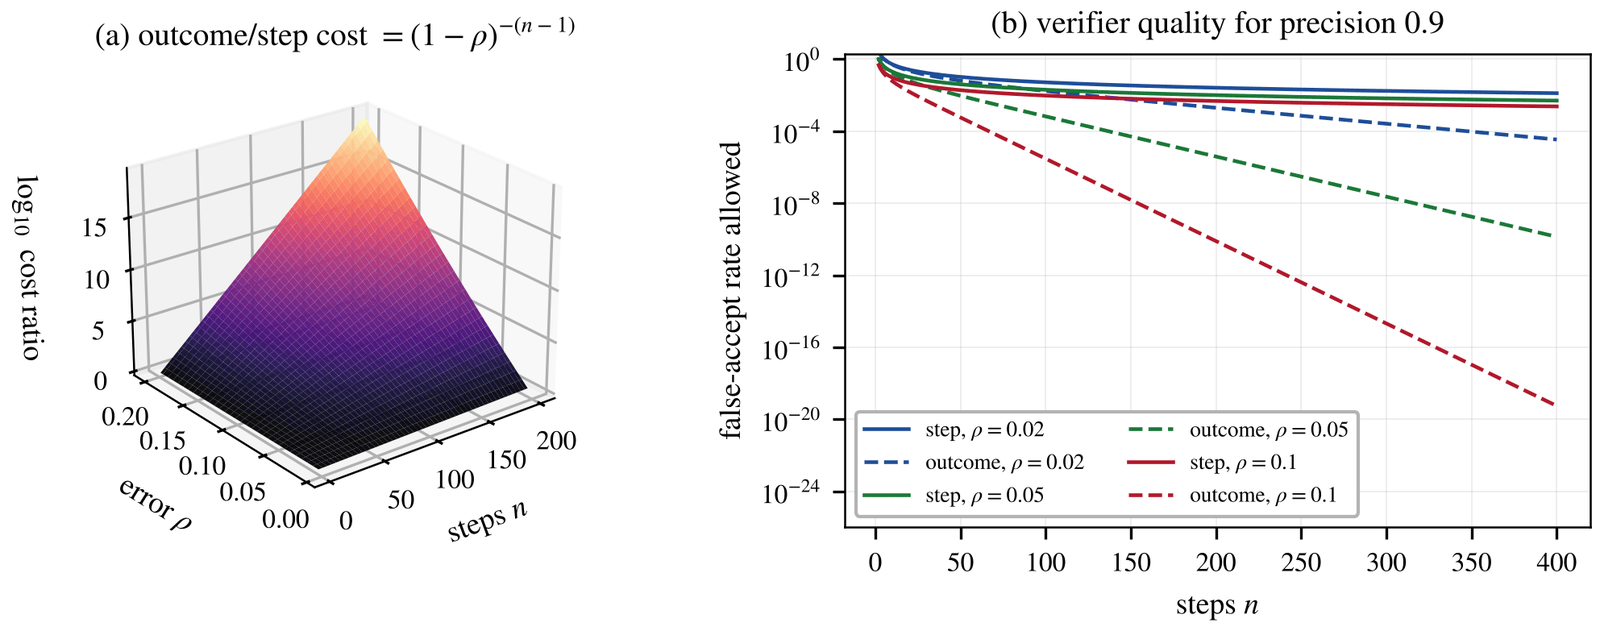
\includegraphics[width=0.98\textwidth]{figures/fig_gating}
\caption{Theorem~\ref{thm:gating}. (a) The ratio $(1-\rho)^{-(n-1)}$ of the expected costs of outcome and step gating with perfect checks, on a logarithmic scale, for up to two hundred steps and error rates $\rho\le0.2$. (b) The false acceptance rate a check may have to reach precision $0.9$ with $\eta=0$: for step gating (solid lines and shaded bands between the sufficient and the necessary rate of part (iv)) it decreases like $1/n$, for outcome gating (dashed) like $(1-\rho)^{n}$.}
\label{fig:gating}
\end{figure*}

\begin{figure*}[t]
\centering
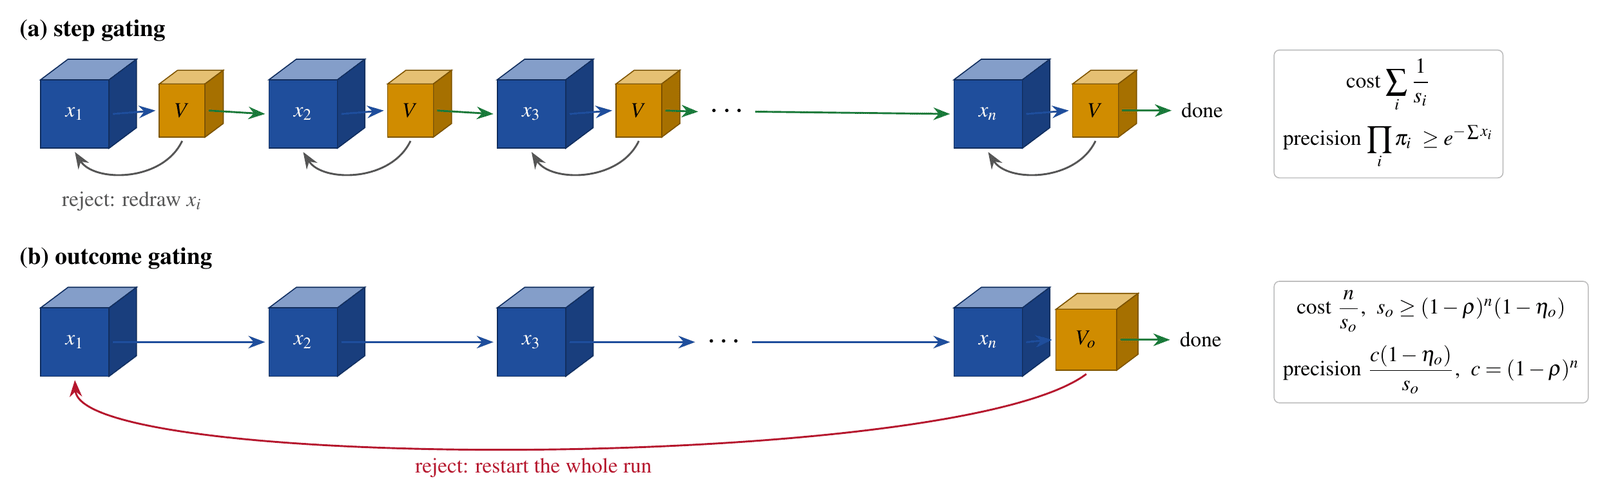
\includegraphics[width=0.94\textwidth]{figures/fig_gatingflow}
\caption{The two protocols of Theorem~\ref{thm:gating}. (a) Step gating: each step is generated and checked, and regenerated until accepted; the cost is $\sum1/s_{i}$ and the precision $\prod\pi_{i}\ge e^{-\sum x_{i}}$. (b) Outcome gating: the chain is generated to the end and checked once, and regenerated until accepted; the acceptance probability is at least $(1-\rho)^{n}(1-\eta_{o})$, the cost is $n/s_{o}$ and the precision $c(1-\eta_{o})/s_{o}$.}
\label{fig:gatingflow}
\end{figure*}

\begin{remark}[Relation to learning from outcomes]
Jia, Rakhlin and Xie proved that learning a policy from outcome rewards is statistically no harder than learning it from step rewards, up to polynomial factors in the horizon \cite{JRX25}. Theorem~\ref{thm:gating} is about a different cost, that of certifying a chain with checks that are already given, and the two results are compatible: a learner may extract as much from outcomes as from steps, while a certifier that sees only outcomes pays exponentially in retries and in the reliability its check must have. Rohatgi and coauthors observe the same amplification of verifier error along a generation from the side of sampling \cite{RSS25}.
\end{remark}
